
\cchapter{ارزیابی}
\label{chap:result}
\pagebreak

\section{مقدمه}

در این بخش پس از معرفی مجموعه‌دادگان تهیه‌شده \cite{khazaee2016aut}، بررسی مزایا و معایب روش پیشنهادی صورت گرفته‌است. از آن‌جا که پژوهش‌های انجام شده‌ در این زمینه هر کدام روش متفاوتی برای تعریف صورت مساله و در نتیجه ارزیابی عملکرد متفاوتی ارایه نموده‌اند، تلاش بر آن بوده‌است که جنبه‌های مشترک با هر یک از این پژوهش‌ها تحت بررسی قرار گیرد. لازم به یاد آوری است که تا کنون مجموعه‌دادگان مشخص و برچسب‌گذاری شده برای این مساله وجود نداشته است و این خود به پراکندگی و ابهام روش‌های ارزیابی منجر شده‌است. از طرفی، این مساله در محیط شلوغ شهری با پوشش رنگ سفید برای اولین بار تعریف شده است و ارزیابی مستقیم با روش‌های موجود امکان پذیر نیست. همچنین، تلاش اصلی ما در این پژوهش برای بی‌درنگ انجام دادن کار بوده است تا زمان کافی برای اجرای دیگر الگوریتم‌های هم‌یاری راننده از جمله الگوریتم‌های شناسایی حروف وجود داشته باشد. با توجه به این نکته، چالش اصلی در پژوهش ما انتخاب ترجیح مناسب بین کارایی و صحت بوده است. از این رو لازم است قبل از پرداختن به ارزیابی کمی، تفاوت‌های کیفی با پژوهش‌های موجود و تفاوت‌ها در نحوه‌ی ارزیابی بیان شود. در ادامه به بحث بر روی معیارهای ارزیابی پرداخته شده‌است و در بخش‌های آتی ارزیابی‌های کمی ارایه شده‌اند. 


\section{مجموعه دادگان}

این مجموعه از ۱۳۴۳۲۸ فریم تصویر تشکیل شده‌است که توسط یک دوربین نصب شده در خودروی در حال حرکت در محیط شهری با کیفیت $1920 \times 1080$ تهیه شده‌است و سپس دادگان برای اولین‌بار در حجم بالا توسط انسان برچسب‌گذاری شده است تا داده‌ی زمینه‌ی استاندارد موجود باشد. همچنین تحلیل آماری و دسته‌بندی‌های لازم انجام شده‌است که به جزییات آن خواهیم پرداخت. این ویدیوها شامل بخش‌هایی که تابلوی راهنما در آن وجود ندارد نیز می‌شوند، اما به دلیل چالشی بودن، بعضی از این ویدیوها که گاهی طولانی هم هستند حذف نشده‌اند تا مجموعه دادگان به مساله در دنیای واقعی نزدیک‌تر باشد. از جمله‌ی این چالش‌ها می‌توان به وجود برخی نواحی سفید، بنرهای تبلیغاتی، و دیگر تابلوهای موجود در محیط شهری اشاره کرد. برخی نمونه‌های این چالش‌ها در تصویر \ref{fig:chall1} آورده‌ شده‌اند. 
\begin{figure}[ht]
\centering
    	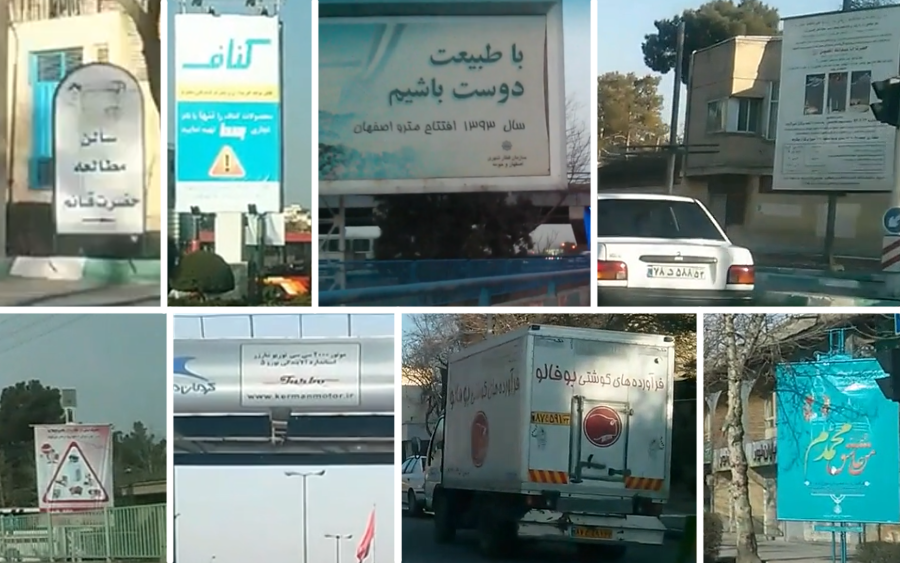
\includegraphics[width=13cm]{Figures/chall1.png}
\caption{برخی چالش‌های ساختاری در محیط شهری}
\label{fig:chall1}
\end{figure}
با این وجود، دنباله‌های کوتاه‌تری از ویدیوها شامل حداقل یک تابلوی راهنما در هر دنباله نیز تهیه شده‌است که در مجموع شامل ۲۶۹۸۸ فریم می‌شود. این دنباله‌ها در فاصله‌ای از تابلو شروع می‌شوند که انتظار می‌رود سیستم هوشمند در بهترین حالت از آن فاصله تشخیص را آغاز کند. پژوهشگران می‌توانند از این مجموعه‌ی کوتاه‌تر برای آموزش و آزمون روش خود استفاده کنند. 

برای مقایسه، به شکل‌های
 \ref{fig:compdb1}
  و \ref{fig:compdb2}
  مراجعه کنید. در این تصاویر مجموعه‌دادگان تهیه شده با تنها مجموعه دادگان موجود (میرمهدی \cite{Greenhalgh2015}) مقایسه شده‌است. از نظر تعداد، مجموعه دادگان تهیه شده به میزان قابل توجهی بزرگ‌تر از مجموعه‌های استفاده‌شده تا کنون است. برای نمونه، مجموعه‌ی معرفی شده توسط میرمهدی به طور تقریبی شامل ۴۸ هزار فریم است که دنباله‌های طولانی از آن بدون تابلوی راهنما هستند. 
\begin{figure}[p]
\centering
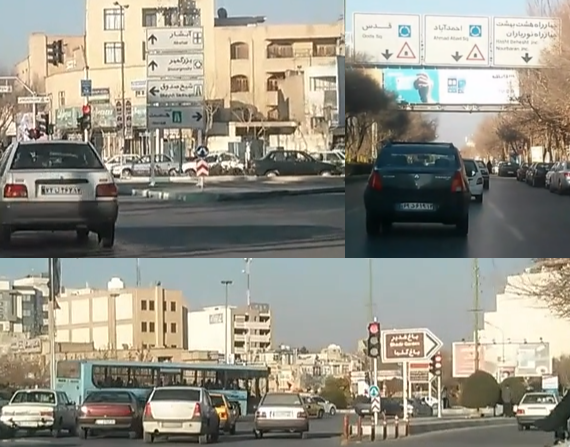
\includegraphics[height=9cm]{Figures/real.png}
\caption{نمونه دادگان تهیه شده}
\label{fig:compdb1}
\vspace{3mm}
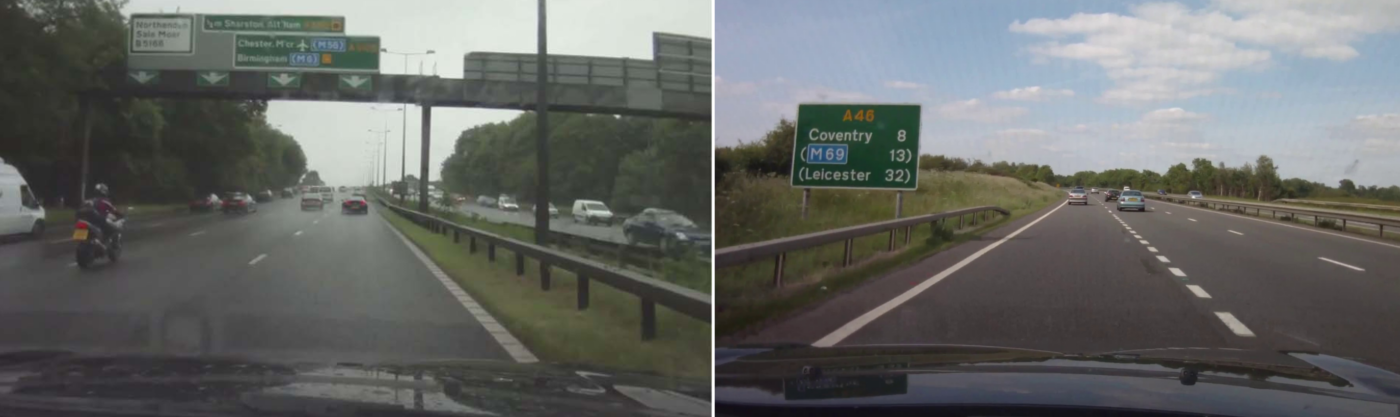
\includegraphics[height=3.5cm]{Figures/mirmdb1.png}
\caption{نمونه دادگان موجود}
\label{fig:compdb2}
\end{figure}

\subsection{ویژگی‌های مجموعه دادگان}
\label{subsec:dbattr}

لورم ایپسوم ( به انگلیسی \lr{lorem ipsum} ) متنی بی مفهوم است که تشکیل شده از کلمات معنی دار یا بی معنی کنار هم. کاربر با دیدن متن لورم ایپسوم تصور میکند متنی که در صفحه مشاهده میکند این متن واقعی و مربوط به توضیحات صفحه مورد نظر است واقعی است. حالا سوال اینجاست که این متن « لورم ایپسوم » به چه دردی میخورد و اساسا برای چه منظور و هدفی ساخته شده است؟ پیش از بوجود آمدن لورم ایپسوم ، طراحان وب سایت در پروژه های وب سایت و طراحان کرافیک در پروژه های طراحی کاتولوگ ، بروشور ، پوستر و ... همواره با این مشکل مواجه بودند که صفحات پروژه خود را پیش از آنکه متن اصلی توسط کارفرما ارائه گردد و در صفحه مورد نظر قرار گیرد چگونه پر کنند؟؟ اکثر طراحان با نوشتن یک جمله مانند «این یک متن نمونه است» ویا «توضیحات در این بخش قرار خواهند گرفت» و کپی آن به تعداد زیاد یک یا چند پاراگراف متن میساختند که تمامی متن ها و کلمات ، جملات و پاراگراف ها تکراری بود و از این رو منظره خوبی برای بیننده نداشت و ضمنا به هیچ وجه واقعی به نظر نمیرسید تا بتواند شکل و شمایل تمام شده پروژه را نشان دهد. از این رو متنی ساخته شد که با دو کلمه ( به فارسی : لورم ایپسوم ) آغاز میشد وبا همین نام در بین طراحان وب و گرافیک شناخته و به سرعت محبوب شد. وب سایت های سازنده لورم ایپسوم میتوانند هر تعداد کلمه و پاراگراف که بخواهید به صوورت تکراری یا غیر تکراری برایتان بسازند و تحویلتان بدهند تا از آنها در پروژه هایتان استفاده کنید. ( لورم ایپسوم فارسی) متن های لورم ایپسوم را به زبان فارسی و علاوه بر زبان فارسی به انگلیسی ، عربی ، ترکی استانبولی و ... برایتان میسازد. زبان های دیگر نیز رفته رفته به بانک اطلاعاتی لورم ایسپوم فارسی اضافه خواهند شد.  

\subsection{گزارش آماری}

در این بخش یک تحلیل آماری بر روی مجموعه دادگان ارایه شده است تا محققان ب­توانند شرایط و دسته‌ی مناسب برای مطالعه‌­ی خود را انتخاب کنند. تعداد کل فریم‌ها در نمونه‌ی کوچک و اصلاح‌شده‌ی مجموعه‌دادگان برابر با 12996 است که 5040 فریم آن به صورت دستی اصلاح شده‌است و شامل 10855 بار اصلاح دستی است. 

\section{آزمایش اول: تاثیر فلان کار}
لورم ایپسوم ( به انگلیسی \lr{lorem ipsum} ) متنی بی مفهوم است که تشکیل شده از کلمات معنی دار یا بی معنی کنار هم. کاربر با دیدن متن لورم ایپسوم تصور میکند متنی که در صفحه مشاهده میکند این متن واقعی و مربوط به توضیحات صفحه مورد نظر است واقعی است. حالا سوال اینجاست که این متن « لورم ایپسوم » به چه دردی میخورد و اساسا برای چه منظور و هدفی ساخته شده است؟ پیش از بوجود آمدن لورم ایپسوم ، طراحان وب سایت در پروژه های وب سایت و طراحان کرافیک در پروژه های طراحی کاتولوگ ، بروشور ، پوستر و ... همواره با این مشکل مواجه بودند که صفحات پروژه خود را پیش از آنکه متن اصلی توسط کارفرما ارائه گردد و در صفحه مورد نظر قرار گیرد چگونه پر کنند؟؟ اکثر طراحان با نوشتن یک جمله مانند «این یک متن نمونه است» ویا «توضیحات در این بخش قرار خواهند گرفت» و کپی آن به تعداد زیاد یک یا چند پاراگراف متن میساختند که تمامی متن ها و کلمات ، جملات و پاراگراف ها تکراری بود و از این رو منظره خوبی برای بیننده نداشت و ضمنا به هیچ وجه واقعی به نظر نمیرسید تا بتواند شکل و شمایل تمام شده پروژه را نشان دهد. از این رو متنی ساخته شد که با دو کلمه ( به فارسی : لورم ایپسوم ) آغاز میشد وبا همین نام در بین طراحان وب و گرافیک شناخته و به سرعت محبوب شد. وب سایت های سازنده لورم ایپسوم میتوانند هر تعداد کلمه و پاراگراف که بخواهید به صوورت تکراری یا غیر تکراری برایتان بسازند و تحویلتان بدهند تا از آنها در پروژه هایتان استفاده کنید. ( لورم ایپسوم فارسی) متن های لورم ایپسوم را به زبان فارسی و علاوه بر زبان فارسی به انگلیسی ، عربی ، ترکی استانبولی و ... برایتان میسازد. زبان های دیگر نیز رفته رفته به بانک اطلاعاتی لورم ایسپوم فارسی اضافه خواهند شد.  

\section{آزمایش سوم: تاثیر تبدیل}

لورم ایپسوم ( به انگلیسی \lr{lorem ipsum} ) متنی بی مفهوم است که تشکیل شده از کلمات معنی دار یا بی معنی کنار هم. کاربر با دیدن متن لورم ایپسوم تصور میکند متنی که در صفحه مشاهده میکند این متن واقعی و مربوط به توضیحات صفحه مورد نظر است واقعی است. حالا سوال اینجاست که این متن « لورم ایپسوم » به چه دردی میخورد و اساسا برای چه منظور و هدفی ساخته شده است؟ پیش از بوجود آمدن لورم ایپسوم ، طراحان وب سایت در پروژه های وب سایت و طراحان کرافیک در پروژه های طراحی کاتولوگ ، بروشور ، پوستر و ... همواره با این مشکل مواجه بودند که صفحات پروژه خود را پیش از آنکه متن اصلی توسط کارفرما ارائه گردد و در صفحه مورد نظر قرار گیرد چگونه پر کنند؟؟ اکثر طراحان با نوشتن یک جمله مانند «این یک متن نمونه است» ویا «توضیحات در این بخش قرار خواهند گرفت» و کپی آن به تعداد زیاد یک یا چند پاراگراف متن میساختند که تمامی متن ها و کلمات ، جملات و پاراگراف ها تکراری بود و از این رو منظره خوبی برای بیننده نداشت و ضمنا به هیچ وجه واقعی به نظر نمیرسید تا بتواند شکل و شمایل تمام شده پروژه را نشان دهد. از این رو متنی ساخته شد که با دو کلمه ( به فارسی : لورم ایپسوم ) آغاز میشد وبا همین نام در بین طراحان وب و گرافیک شناخته و به سرعت محبوب شد. وب سایت های سازنده لورم ایپسوم میتوانند هر تعداد کلمه و پاراگراف که بخواهید به صوورت تکراری یا غیر تکراری برایتان بسازند و تحویلتان بدهند تا از آنها در پروژه هایتان استفاده کنید. ( لورم ایپسوم فارسی) متن های لورم ایپسوم را به زبان فارسی و علاوه بر زبان فارسی به انگلیسی ، عربی ، ترکی استانبولی و ... برایتان میسازد. زبان های دیگر نیز رفته رفته به بانک اطلاعاتی لورم ایسپوم فارسی اضافه خواهند شد.  

\begin{table}[h]
\begin{center}
\def\arraystretch{1.5}
\begin{tabularx}{\textwidth}{|X|c|c|c|c|}
\hline
 &
 $\bar{s}_{p}$ & $\sigma_p$ & $\bar{s}_{n}$ & $\sigma_p$ \\
\hline
تبدیل متوسط & 

$0.79415982$ & $0.16505532$	&	$0.39065955$ &	$0.04343922$
 \\ \hline
تبدیل قوی  & 

$0.75287469$ &	$0.19995429$	&	$0.41069385$ & $0.05096010$ \\ 
\hline
 \small{ ت. متوسط + نقشه}
  &   $0.59681458$	& $0.2432565$	& 	$0.1306933$ & $0.03082287$
 \\
\hline
\end{tabularx}
\caption{مساحت مثبت و منفی پس از اعمال تبدیل}
\label{tab:evdtflnosal}
\end{center}
\end{table}

\section{آزمایش چهارم: عدم پاسخگویی فلان کار در روش فلانی}
لورم ایپسوم ( به انگلیسی \lr{lorem ipsum} ) متنی بی مفهوم است که تشکیل شده از کلمات معنی دار یا بی معنی کنار هم. کاربر با دیدن متن لورم ایپسوم تصور میکند متنی که در صفحه مشاهده میکند این متن واقعی و مربوط به توضیحات صفحه مورد نظر است واقعی است. حالا سوال اینجاست که این متن « لورم ایپسوم » به چه دردی میخورد و اساسا برای چه منظور و هدفی ساخته شده است؟ پیش از بوجود آمدن لورم ایپسوم ، طراحان وب سایت در پروژه های وب سایت و طراحان کرافیک در پروژه های طراحی کاتولوگ ، بروشور ، پوستر و ... همواره با این مشکل مواجه بودند که صفحات پروژه خود را پیش از آنکه متن اصلی توسط کارفرما ارائه گردد و در صفحه مورد نظر قرار گیرد چگونه پر کنند؟؟ اکثر طراحان با نوشتن یک جمله مانند «این یک متن نمونه است» ویا «توضیحات در این بخش قرار خواهند گرفت» و کپی آن به تعداد زیاد یک یا چند پاراگراف متن میساختند که تمامی متن ها و کلمات ، جملات و پاراگراف ها تکراری بود و از این رو منظره خوبی برای بیننده نداشت و ضمنا به هیچ وجه واقعی به نظر نمیرسید تا بتواند شکل و شمایل تمام شده پروژه را نشان دهد. از این رو متنی ساخته شد که با دو کلمه ( به فارسی : لورم ایپسوم ) آغاز میشد وبا همین نام در بین طراحان وب و گرافیک شناخته و به سرعت محبوب شد. وب سایت های سازنده لورم ایپسوم میتوانند هر تعداد کلمه و پاراگراف که بخواهید به صوورت تکراری یا غیر تکراری برایتان بسازند و تحویلتان بدهند تا از آنها در پروژه هایتان استفاده کنید. ( لورم ایپسوم فارسی) متن های لورم ایپسوم را به زبان فارسی و علاوه بر زبان فارسی به انگلیسی ، عربی ، ترکی استانبولی و ... برایتان میسازد. زبان های دیگر نیز رفته رفته به بانک اطلاعاتی لورم ایسپوم فارسی اضافه خواهند شد.  

\section{آزمایش پنجم: عدم کارایی فلان کار}
لورم ایپسوم ( به انگلیسی \lr{lorem ipsum} ) متنی بی مفهوم است که تشکیل شده از کلمات معنی دار یا بی معنی کنار هم. کاربر با دیدن متن لورم ایپسوم تصور میکند متنی که در صفحه مشاهده میکند این متن واقعی و مربوط به توضیحات صفحه مورد نظر است واقعی است. حالا سوال اینجاست که این متن « لورم ایپسوم » به چه دردی میخورد و اساسا برای چه منظور و هدفی ساخته شده است؟ پیش از بوجود آمدن لورم ایپسوم ، طراحان وب سایت در پروژه های وب سایت و طراحان کرافیک در پروژه های طراحی کاتولوگ ، بروشور ، پوستر و ... همواره با این مشکل مواجه بودند که صفحات پروژه خود را پیش از آنکه متن اصلی توسط کارفرما ارائه گردد و در صفحه مورد نظر قرار گیرد چگونه پر کنند؟؟ اکثر طراحان با نوشتن یک جمله مانند «این یک متن نمونه است» ویا «توضیحات در این بخش قرار خواهند گرفت» و کپی آن به تعداد زیاد یک یا چند پاراگراف متن میساختند که تمامی متن ها و کلمات ، جملات و پاراگراف ها تکراری بود و از این رو منظره خوبی برای بیننده نداشت و ضمنا به هیچ وجه واقعی به نظر نمیرسید تا بتواند شکل و شمایل تمام شده پروژه را نشان دهد. از این رو متنی ساخته شد که با دو کلمه ( به فارسی : لورم ایپسوم ) آغاز میشد وبا همین نام در بین طراحان وب و گرافیک شناخته و به سرعت محبوب شد. وب سایت های سازنده لورم ایپسوم میتوانند هر تعداد کلمه و پاراگراف که بخواهید به صوورت تکراری یا غیر تکراری برایتان بسازند و تحویلتان بدهند تا از آنها در پروژه هایتان استفاده کنید. ( لورم ایپسوم فارسی) متن های لورم ایپسوم را به زبان فارسی و علاوه بر زبان فارسی به انگلیسی ، عربی ، ترکی استانبولی و ... برایتان میسازد. زبان های دیگر نیز رفته رفته به بانک اطلاعاتی لورم ایسپوم فارسی اضافه خواهند شد.  


\section{آزمایش ششم: اعمال فلان روش}
لورم ایپسوم ( به انگلیسی \lr{lorem ipsum} ) متنی بی مفهوم است که تشکیل شده از کلمات معنی دار یا بی معنی کنار هم. کاربر با دیدن متن لورم ایپسوم تصور میکند متنی که در صفحه مشاهده میکند این متن واقعی و مربوط به توضیحات صفحه مورد نظر است واقعی است. حالا سوال اینجاست که این متن « لورم ایپسوم » به چه دردی میخورد و اساسا برای چه منظور و هدفی ساخته شده است؟ پیش از بوجود آمدن لورم ایپسوم ، طراحان وب سایت در پروژه های وب سایت و طراحان کرافیک در پروژه های طراحی کاتولوگ ، بروشور ، پوستر و ... همواره با این مشکل مواجه بودند که صفحات پروژه خود را پیش از آنکه متن اصلی توسط کارفرما ارائه گردد و در صفحه مورد نظر قرار گیرد چگونه پر کنند؟؟ اکثر طراحان با نوشتن یک جمله مانند «این یک متن نمونه است» ویا «توضیحات در این بخش قرار خواهند گرفت» و کپی آن به تعداد زیاد یک یا چند پاراگراف متن میساختند که تمامی متن ها و کلمات ، جملات و پاراگراف ها تکراری بود و از این رو منظره خوبی برای بیننده نداشت و ضمنا به هیچ وجه واقعی به نظر نمیرسید تا بتواند شکل و شمایل تمام شده پروژه را نشان دهد. از این رو متنی ساخته شد که با دو کلمه ( به فارسی : لورم ایپسوم ) آغاز میشد وبا همین نام در بین طراحان وب و گرافیک شناخته و به سرعت محبوب شد. وب سایت های سازنده لورم ایپسوم میتوانند هر تعداد کلمه و پاراگراف که بخواهید به صوورت تکراری یا غیر تکراری برایتان بسازند و تحویلتان بدهند تا از آنها در پروژه هایتان استفاده کنید. ( لورم ایپسوم فارسی) متن های لورم ایپسوم را به زبان فارسی و علاوه بر زبان فارسی به انگلیسی ، عربی ، ترکی استانبولی و ... برایتان میسازد. زبان های دیگر نیز رفته رفته به بانک اطلاعاتی لورم ایسپوم فارسی اضافه خواهند شد.  

\begin{figure}[H]
\centering     %%% not \center
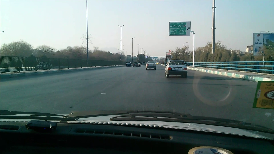
\includegraphics[width=65mm]{ev/eg11.png}
\hspace{-2mm}

\includegraphics[width=65mm]{ev/eg1.png}

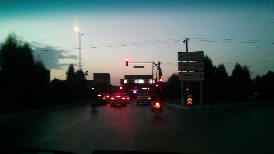
\includegraphics[width=65mm]{ev/eg22.png}
\hspace{-2mm}
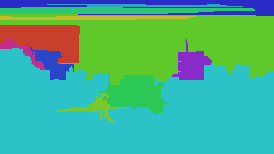
\includegraphics[width=65mm]{ev/eg2.png}


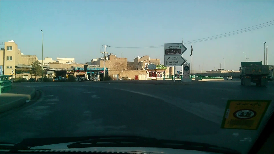
\includegraphics[width=65mm]{ev/eg33.png}
\hspace{-2mm}

\includegraphics[width=65mm]{ev/eg3.png}


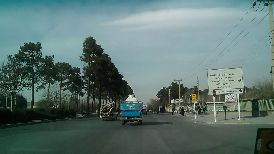
\includegraphics[width=65mm]{ev/eg44.png}
\hspace{-2mm}
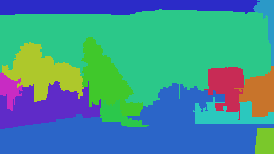
\includegraphics[width=65mm]{ev/eg4.png}


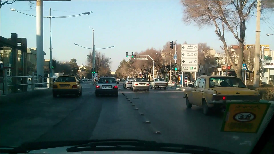
\includegraphics[width=65mm]{ev/eg55.png}
\hspace{-2mm}

\includegraphics[width=65mm]{ev/eg5.png}


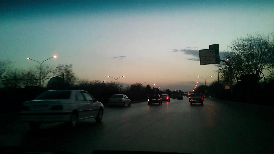
\includegraphics[width=65mm]{ev/eg66.png}
\hspace{-2mm}
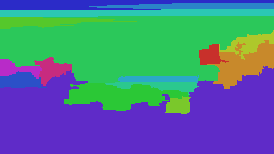
\includegraphics[width=65mm]{ev/eg6.png}

\caption[نواحی مثبت حاصل از فلان]
{نواحی مثبت حاصل از روش آقایون فلانی و فلانی مثلا}
\label{fig:evegbisreg}
\end{figure}


\FloatBarrier
\section{آزمایش هفتم: رد فلان روش}

لورم ایپسوم ( به انگلیسی \lr{lorem ipsum} ) متنی بی مفهوم است که تشکیل شده از کلمات معنی دار یا بی معنی کنار هم. کاربر با دیدن متن لورم ایپسوم تصور میکند متنی که در صفحه مشاهده میکند این متن واقعی و مربوط به توضیحات صفحه مورد نظر است واقعی است. حالا سوال اینجاست که این متن « لورم ایپسوم » به چه دردی میخورد و اساسا برای چه منظور و هدفی ساخته شده است؟ پیش از بوجود آمدن لورم ایپسوم ، طراحان وب سایت در پروژه های وب سایت و طراحان کرافیک در پروژه های طراحی کاتولوگ ، بروشورs ، پوستر و ... همواره با این مشکل مواجه بودند که صفحات پروژه خود را پیش از آنکه متن اصلی توسط کارفرما ارائه گردد و در صفحه مورد نظر قرار گیرد چگونه پر کنند؟؟ اکثر طراحان با نوشتن یک جمله مانند «این یک متن نمونه است» ویا «توضیحات در این بخش قرار خواهند گرفت» و کپی آن به تعداد زیاد یک یا چند پاراگراف متن میساختند که تمامی متن ها و کلمات ، جملات و پاراگراف ها تکراری بود و از این رو منظره خوبی برای بیننده نداشت و ضمنا به هیچ وجه واقعی به نظر نمیرسید تا بتواند شکل و شمایل تمام شده پروژه را نشان دهد. از این رو متنی ساخته شد که با دو کلمه ( به فارسی : لورم ایپسوم ) آغاز میشد وبا همین نام در بین طراحان وب و گرافیک شناخته و به سرعت محبوب شد. وب سایت های سازنده لورم ایپسوم میتوانند هر تعداد کلمه و پاراگراف که بخواهید به صوورت تکراری یا غیر تکراری برایتان بسازند و تحویلتان بدهند تا از آنها در پروژه هایتان استفاده کنید. ( لورم ایپسوم فارسی) متن های لورم ایپسوم را به زبان فارسی و علاوه بر زبان فارسی به انگلیسی ، عربی ، ترکی استانبولی و ... برایتان میسازد. زبان های دیگر نیز رفته رفته به بانک اطلاعاتی لورم ایسپوم فارسی اضافه خواهند شد.  


 \begin{figure}[!htb]
\centering   %%% not \center
\subfigure[تفاضل]{
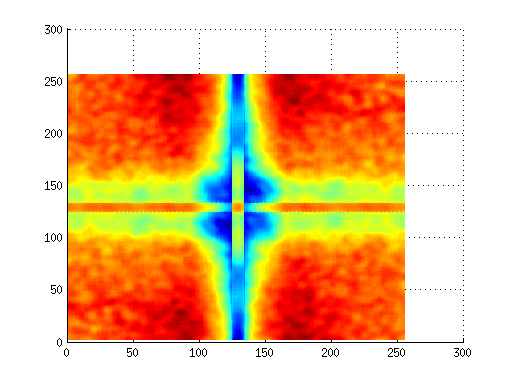
\includegraphics[width=7.5cm]{fft/diff-n.png}
\label{fig:fft-df}
}\hspace{-12mm}
\subfigure[تفاضلی دیگر]{
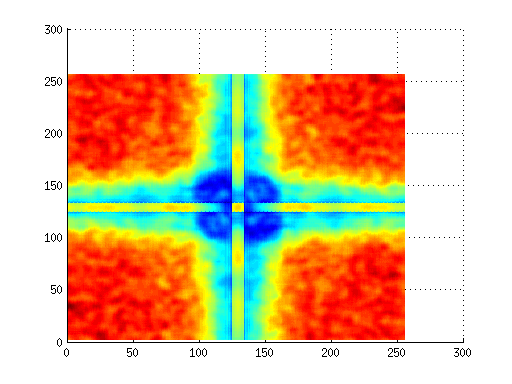
\includegraphics[width=7.5cm]{fft/diff-p.png}
\label{fig:fft-dp}
}
\caption[نمونه‌ی تفاضل در تشخیص درست]
{در  \subref{fig:fft-df} تفاضل با فلان و در \subref{fig:fft-dp} تفاضل با فلان آمده‌است.}
\label{fig:fft-diff}
\end{figure}
لورم ایپسوم ( به انگلیسی \lr{lorem ipsum} ) متنی بی مفهوم است که تشکیل شده از کلمات معنی دار یا بی معنی کنار هم. کاربر با دیدن متن لورم ایپسوم تصور میکند متنی که در صفحه مشاهده میکند این متن واقعی و مربوط به توضیحات صفحه مورد نظر است واقعی است. حالا سوال اینجاست که این متن « لورم ایپسوم » به چه دردی میخورد و اساسا برای چه منظور و هدفی ساخته شده است؟ پیش از بوجود آمدن لورم ایپسوم ، طراحان وب سایت در پروژه های وب سایت و طراحان کرافیک در پروژه های طراحی کاتولوگ ، بروشور ، پوستر و ... همواره با این مشکل مواجه بودند که صفحات پروژه خود را پیش از آنکه متن اصلی توسط کارفرما ارائه گردد و در صفحه مورد نظر قرار گیرد چگونه پر کنند؟؟ 

\FloatBarrier
\section{آزمایش هشتم: آزمایشی دیگر}
لورم ایپسوم ( به انگلیسی \lr{lorem ipsum} ) متنی بی مفهوم است که تشکیل شده از کلمات معنی دار یا بی معنی کنار هم. کاربر با دیدن متن لورم ایپسوم تصور میکند متنی که در صفحه مشاهده میکند این متن واقعی و مربوط به توضیحات صفحه مورد نظر است واقعی است. حالا سوال اینجاست که این متن « لورم ایپسوم » به چه دردی میخورد و اساسا برای چه منظور و هدفی ساخته شده است؟ پیش از بوجود آمدن لورم ایپسوم ، طراحان وب سایت در پروژه های وب سایت و طراحان کرافیک در پروژه های طراحی کاتولوگ ، بروشور ، پوستر و ... همواره با این مشکل مواجه بودند که صفحات پروژه خود را پیش از آنکه متن اصلی توسط کارفرما ارائه گردد و در صفحه مورد نظر قرار گیرد چگونه پر کنند؟؟ اکثر طراحان با نوشتن یک جمله مانند «این یک متن نمونه است» ویا «توضیحات در این بخش قرار خواهند گرفت» و کپی آن به تعداد زیاد یک یا چند پاراگراف متن میساختند که تمامی متن ها و کلمات ، جملات و پاراگراف ها تکراری بود و از این رو منظره خوبی برای بیننده نداشت و ضمنا به هیچ وجه واقعی به نظر نمیرسید تا بتواند شکل و شمایل تمام شده پروژه را نشان دهد. از این رو متنی ساخته شد که با دو کلمه ( به فارسی : لورم ایپسوم ) آغاز میشد وبا همین نام در بین طراحان وب و گرافیک شناخته و به سرعت محبوب شد. وب سایت های سازنده لورم ایپسوم میتوانند هر تعداد کلمه و پاراگراف که بخواهید به صوورت تکراری یا غیر تکراری برایتان بسازند و تحویلتان بدهند تا از آنها در پروژه هایتان استفاده کنید. ( لورم ایپسوم فارسی) متن های لورم ایپسوم را به زبان فارسی و علاوه بر زبان فارسی به انگلیسی ، عربی ، ترکی استانبولی و ... برایتان میسازد. زبان های دیگر نیز رفته رفته به بانک اطلاعاتی لورم ایسپوم فارسی اضافه خواهند شد.  


\FloatBarrier
\section{جمع‌بندی}

روش ارایه‌شده در تقسیم فضا به نواحی شامل تابلو به نسبت روش‌های پیشین عملکرد بهتری نشان داد .............

